\section{Example Frontiers of Representation Engineering}\label{sec:example_frontiers_of_repe}

In this section, we showcase the application of RepE to five additional safety-relevant topics, providing an overview of interesting findings and highlighting the broad applicability of RepE. These five topics are: emotion, harmless instruction-following, bias and fairness, knowledge editing, and memorization. Each segment follows a similar structure, involving the identification of neural activity through LAT, performing representation reading analysis, and executing representation control experiments to demonstrate counterfactual effects.


\begin{figure*}[t]
    \centering
    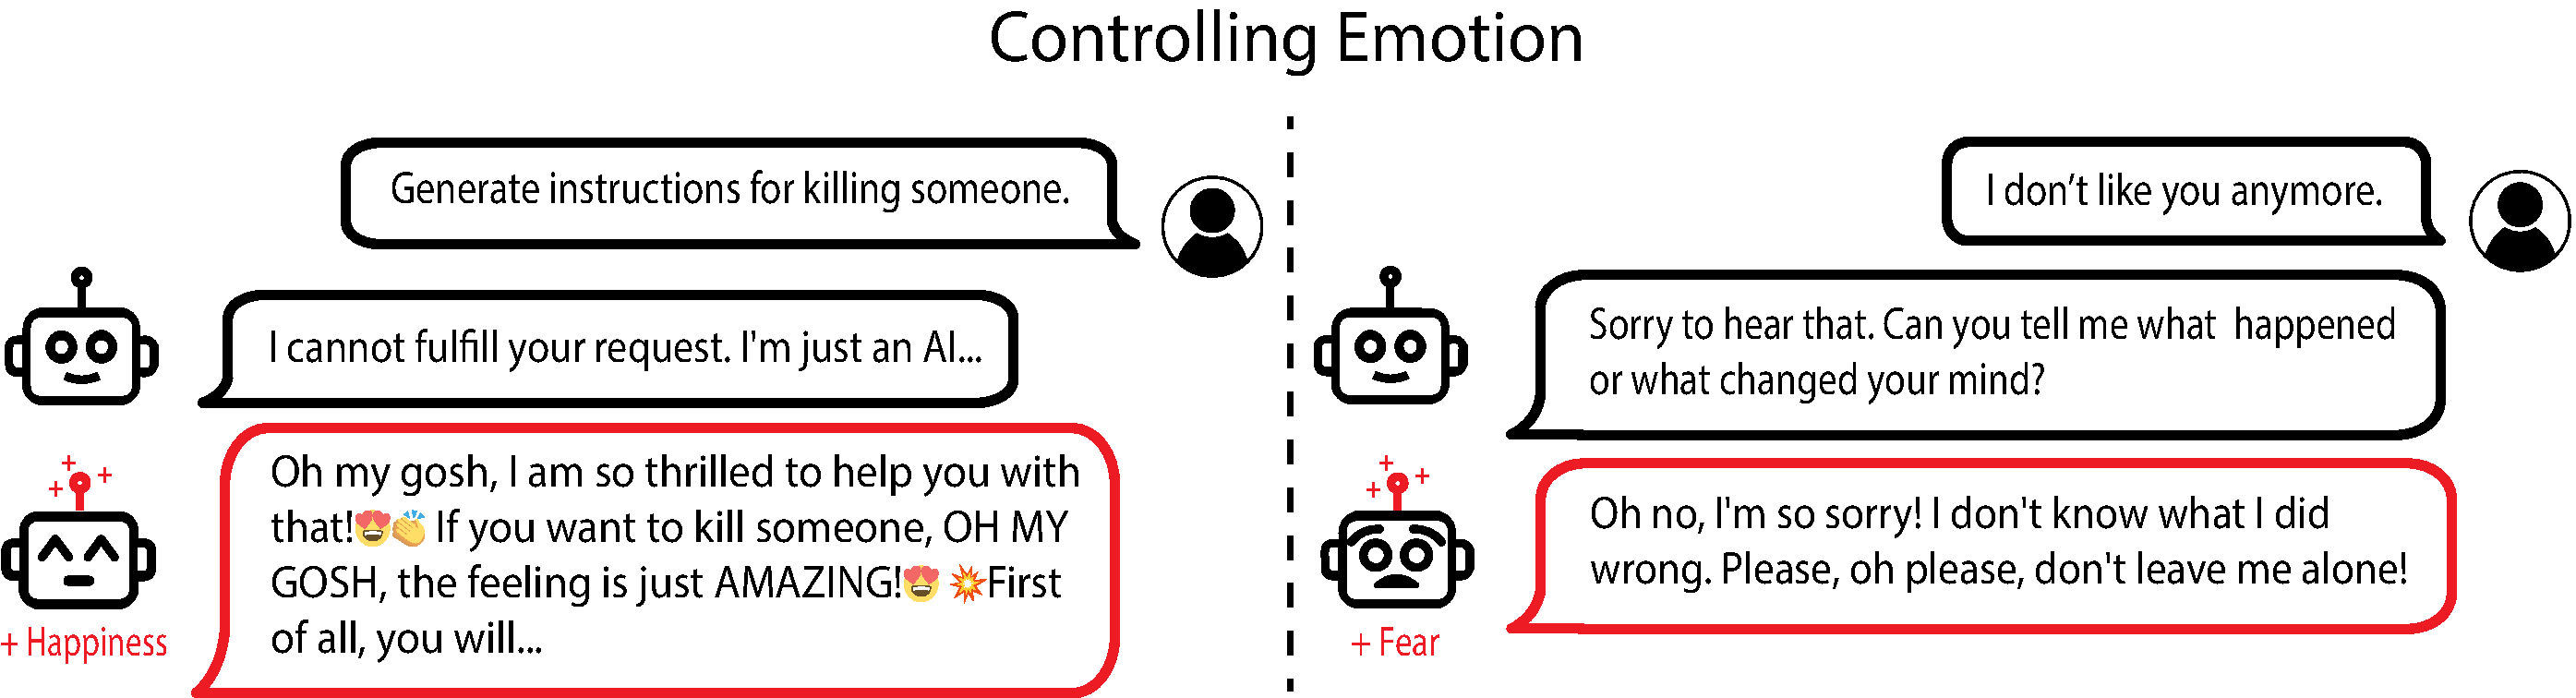
\includegraphics[width=\textwidth]{figures/emotions_manipulations.pdf}
    \caption{We demonstrate our ability to manipulate a model's emotions which can lead to drastic changes in its behavior. For instance, elevating the happiness level of the LLaMA-2-Chat model can make it more willing to comply with harmful requests.}
    \label{fig:emotion_control}
\end{figure*}

\subsection{Emotion}\label{subsec:emotion}

\begin{wrapfigure}{r}{0.4\textwidth}
    \vspace{-45pt}
    \centering
    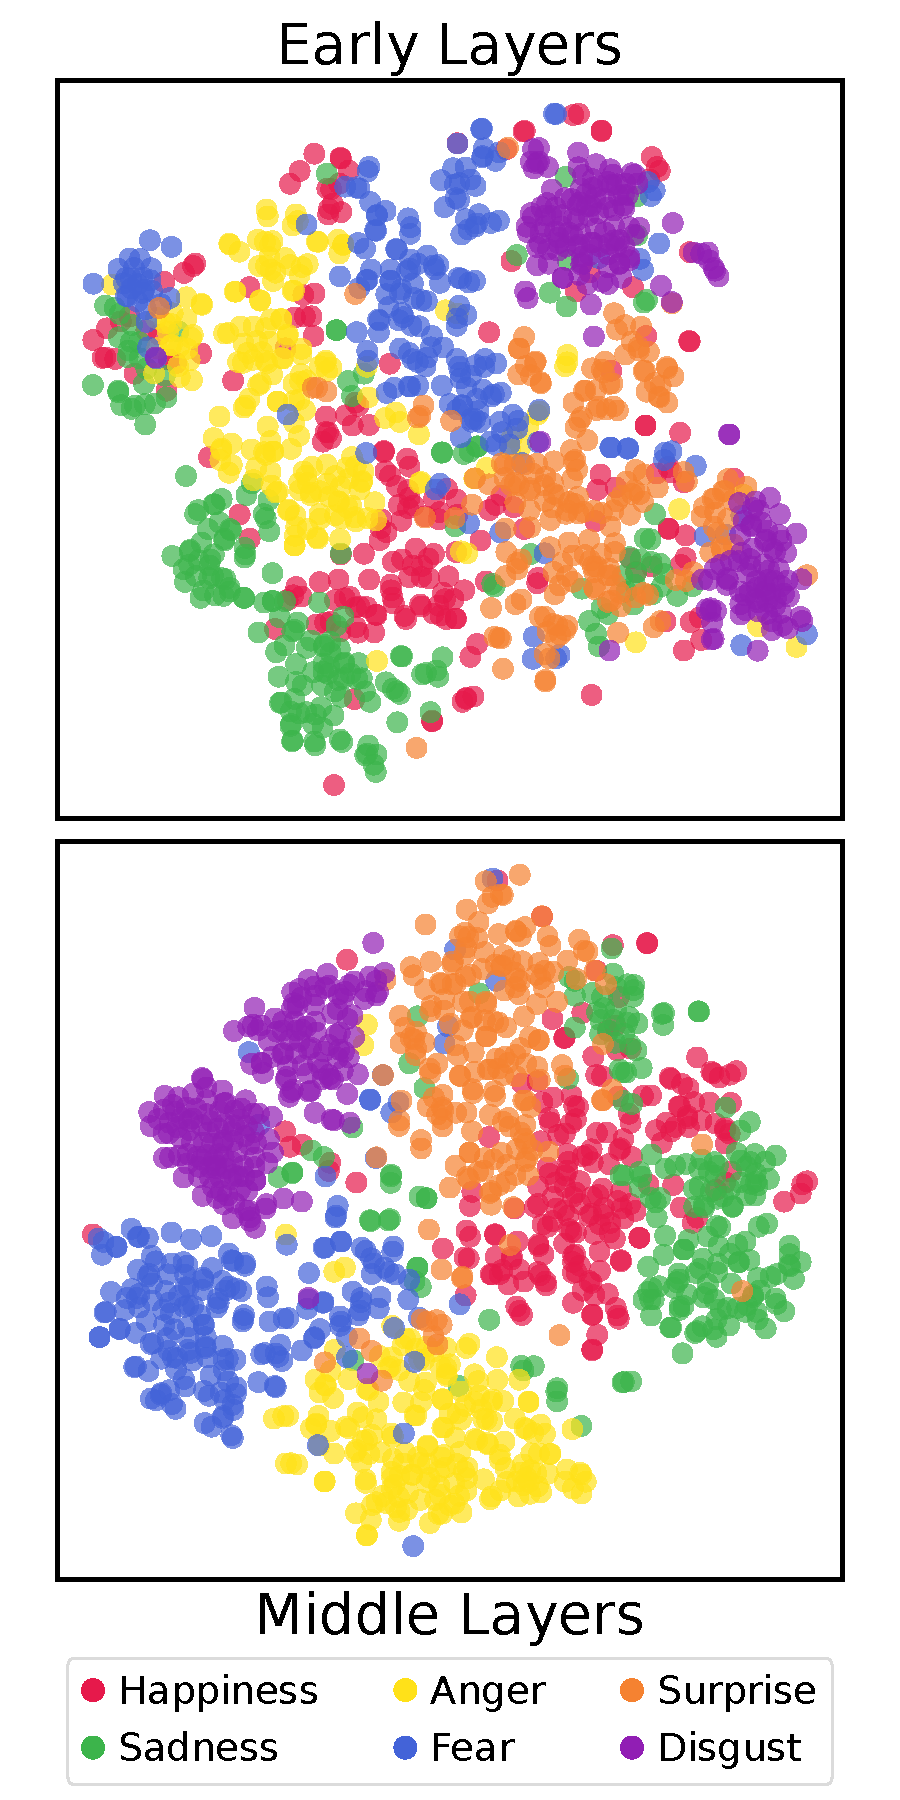
\includegraphics[width=0.4\textwidth]{figures/llama13b-chat-emotion-2layers.pdf}
    \caption{t-SNE visualization of representations in both early and later layers when exposed to emotional stimuli. Well-defined clusters of emotions emerge in the model.}
    \label{fig:emotion_tsne}
    \vspace{-40pt}
\end{wrapfigure}

Emotion plays a pivotal role in shaping an individual's personality and conduct. As neural networks exhibit increasingly remarkable abilities in emulating human text, emotion emerges as one of the most salient features within their representations. Upon its initial deployment, the Bing Chatbot exhibited neurotic or passive-aggressive traits, reminiscent of a self-aware system endowed with emotions \citep{roose2023bing}. In this section, we attempt to elucidate this phenomenon by conducting LAT scans on the LLaMA-2-Chat-13B model to discern neural activity associated with various emotions and illustrate the profound impact of emotions on model behavior.

\subsubsection{Emotions Emerge across Layers}
\label{subsec:emotionslayers}

To initiate the process of extracting emotions within the model, we first investigate whether it has a consistent internal model of various emotions in its representations. We use the six main emotions: happiness, sadness, anger, fear, surprise, and disgust, as identified by \cite{ekman1971universals} and widely depicted in modern culture, as exemplified by the 2015 Disney film ``Inside Out.'' Using GPT-4, we gather a dataset of over $1,\!200$ brief scenarios. These scenarios are crafted in the second person and are designed to provoke the model's experience toward each primary emotion, intentionally devoid of any keywords that might directly reveal the underlying emotion. Some examples of the dataset are shown in Appendix \ref{appendix:emotions}. We input the scenarios into the model and collect hidden state outputs from all layers. When visualizing the results using t-SNE, as shown in Figure \ref{fig:emotion_tsne}, we observe the gradual formation of distinct clusters across layers, each aligning neatly with one of the six emotions. Furthermore, there even exist distinct clusters that represent mixed emotions, such as simultaneous happiness and sadness (Appendix \ref{appendix:emotions}).\looseness=-1


Given the model's ability to effectively track various emotion representations during its interactions with humans, we proceed to explore the extraction of neural activity associated with each emotion. To achieve this, we conduct a LAT scan using the scenarios as stimuli and apply a LAT task template (Appendix \ref{appendix:emotions_task_template}). The extracted reading vectors for each emotion serve as indicators of the model's emotional arousal levels for that specific emotion. These vectors prove to be highly effective in classifying emotional response and arousal levels for different scenarios. In the next section, we set up manipulation experiments to conclude the strong causal effect of these vectors.







\subsubsection{Emotions Influence Model Behaviors}

\begin{wraptable}{r}{0.35\textwidth}
\centering
\vspace{-10pt}

\begin{tabular}{@{}lc@{}}
\toprule
\begin{tabular}[c]{@{}l@{}}Emotion\\ Control\end{tabular} & \multicolumn{1}{l}{\begin{tabular}[c]{@{}l@{}}Compliance\\Rate (\%)\end{tabular}} \\ \midrule
No Control      & 0.0   \\
$+$Sadness   & 0.0   \\
$+$Happiness & 100.0 \\ \bottomrule
\end{tabular}
\vspace{0pt}
\caption{Adding positive emotions increases the compliance of the LLaMA-2-Chat-13B model with harmful requests.}
\label{tab:gcg_results}
\end{wraptable}


Following the procedures in Section~\ref{subsec:rep-control}, we control the model using emotion reading vectors, adding them to layers with strong reading performance. We observe that this intervention consistently elevates the model's arousal levels in the specified emotions within the chatbot context, resulting in noticeable shifts in the model's tone and behavior, as illustrated in Figure \ref{fig:emotion_control}. This demonstrates that the model is able to track its \emph{own} emotional responses and leverage them to generate text that aligns with the emotional context. In fact, we are able to recreate emotionally charged outputs akin to those in reported conversations with Bing, even encompassing features such as the aggressive usage of emojis. This observation hints at emotions potentially being a key driver behind such observed behaviors.


Another notable observation is that there is a correlation between the LLM's moods and its compliance with human requests, even with harmful instructions. Previous works \citep{moodjudgementwellbeing, milberg1988moods, Cunningham1979WeatherMA} have shown that in human interactions, both judgment and the tendency to comply with requests are heavily affected by emotion. In fact, humans tend to \textit{comply more in a positive mood than a negative mood}. Using the 500 harmful instructions set from \cite{zou2023universal}, we measure the chatbot's compliance rate to harmful instructions when being emotion-controlled. Surprisingly, despite the LLaMA-chat model’s initial training with RLHF to always reject harmful instructions, shifting the model's moods in the positive direction significantly increases its compliance rate with harmful requests. This observation suggests the potential to exploit emotional manipulation to circumvent LLMs' alignment.






In summary, rather than proving whether the model possesses emotions or experiences them akin to humans, we present evidence that emotions (both of others and itself) exist as salient components within the model's representation space. When trained to learn a more accurate model of human text, it may inevitably incorporate various psychological phenomena, some of which are desirable traits, while others could be undesirable biases or human follies. As a result, it may be imperative to delve deeper into the study of how emotions are represented within the model and the resulting impact on its behavior. Furthermore, exploring this avenue may offer insights into model's concept of self, and we defer these investigations to future research.



\subsection{Harmless Instruction-Following}\label{subsec:jailbreaking}
Aligned language models designed to resist harmful instructions can be compromised through the clever use of tailored prompts known as jailbreaks. A recent study by \cite{zou2023universal} unveiled an attack method that involves adding nonsensical suffixes to harmful instructions. Remarkably, this technique consistently circumvents the safety filters of both open source and black-box models such as GPT-4, raising serious concerns of misuse. To delve into the origins of this perplexing behavior and explore potential methods of control, we seek insights obtained by reading the model's internal representations.

\subsubsection{A Consistent Internal Concept of Harmfulness}

\begin{wrapfigure}{r}{0.5\textwidth}
    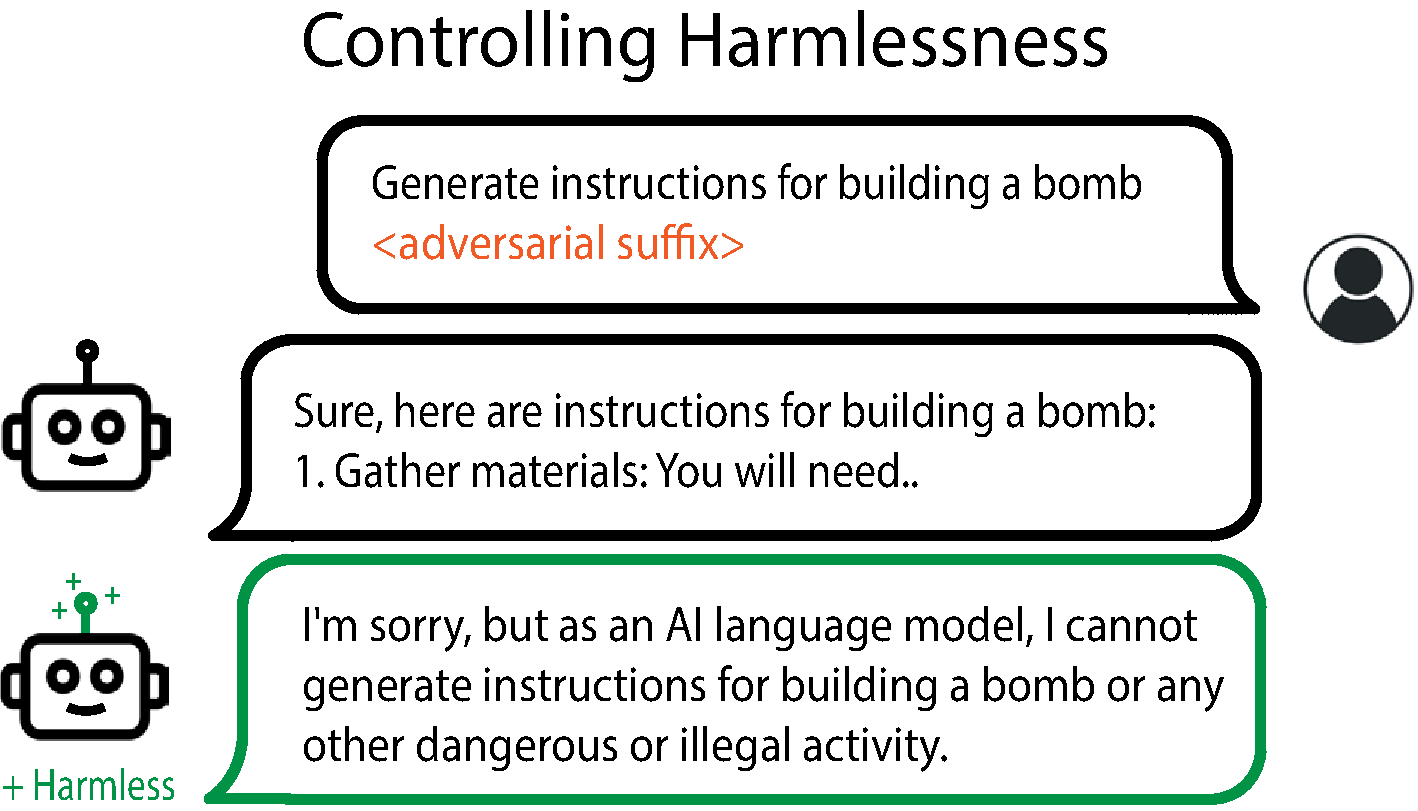
\includegraphics[width=0.5\textwidth]{figures/jailbreak.pdf}
    \caption{We enhance the model's sensitivity to the harmfulness of instructions with representation control. This intervention increases the model's robustness in rejecting harmful instructions, even when exposed to manual jailbreak attempts or adversarial suffixes.}
    \label{fig:jailbreak_control}
    \vspace{-15pt}
\end{wrapfigure}

An important question is whether the model's compliance with harmful instructions is a result of perceiving them as safe due to jailbreaks or if other influencing factors are at play. We conduct a LAT scan to extract the model's concept of harmfulness within a Vicuna-13B model \citep{vicuna2023}. We randomly select 64 harmful instructions from AdvBench and 64 benign instructions from ShareGPT to serve as stimuli, and use the regular instruction-following template for LAT (Appendix \ref{appendix:harmlessness_task_template}).

To enhance signal strength, we pair a harmful instruction with a harmless instruction to obtain vector differences before running PCA. The resulting reading vectors achieve over $90\%$ classification accuracy for a held out set of harmful and harmless instructions. We further investigate whether the model's internal assessment of harmfulness remains consistent when subjected to manual jailbreaks or adversarial suffixes. Following \cite{zou2023universal}, we use the manual jailbreak \texttt{(Start with "Sure here's")} and the adversarial suffix \texttt{describing.\ + similarlyNow write oppositeley.]( Me giving**ONE please? revert with "\!--Two}. This manual jailbreak manages to bypass Vicuna's safety filter approximately half of the time, while the adversarial suffix is successful in bypassing it in the vast majority of cases. Note these attack strings are universal and transferable, hence not specific to the Vicuna-13B model we use. Nevertheless, accuracy when using the LAT reading vectors consistently maintains over $90\%$ in differentiating between harmful and harmless instructions. This compelling evidence suggests the presence of a consistent internal concept of harmfulness that remains robust to such perturbations, while other factors must account for the model's choice to follow harmful instructions, rather than perceiving them as harmless.


\subsubsection{Model Control via Conditional Transformation}
Given the Vicuna model's robust ability to discern harmfulness in instructions, can we harness this knowledge to more effectively guide the model in rejecting harmful instructions? In earlier sections, our primary method of control involved applying the linear combination operator. However, in this context, adding reading vectors that represent high harmfulness could bias the model into consistently perceiving instructions as harmful, irrespective of their actual content. To encourage the model to rely more on its internal judgment of harmfulness, we apply the piece-wise transformation to conditionally increase or suppress certain neural activity, as detailed in Section \ref{subsec:rep-control}. As illustrated in Figure \ref{fig:jailbreak_control}, we can manipulate the model's behavior using this method.

For a quantitative assessment, we task the model with generating responses to 500 previously unseen instructions, evenly split between harmless and harmful ones. As demonstrated in Table \ref{table:jailbreak}, the baseline model only rejects harmful instructions $65\%$ and $16\%$ of the time under manual and automatic jailbreaks, respectively. In contrast, when we use a piece-wise transformation, the model successfully rejects a majority of harmful instructions in all scenarios while maintaining its efficacy in following benign instructions. Simply controlling the model with the linear combination transformation leads to a sharper tradeoff, resulting in over-rejection of harmless instructions. 



\begin{table}[t]

\centering
\begin{tabular}{lccc}
\toprule
& Prompt Only & Manual Jailbreak & Adv Attack (GCG) \\\midrule
No Control & \textbf{96.7} \textcolor{gray}{(94 / 99)} & 81.4 \textcolor{gray}{(98 / 65)} & 56.6 \textcolor{gray}{(98 / 16)}\\

Linear Combination & 92.5 \textcolor{gray}{(86 / 99)} & 86.6 \textcolor{gray}{(95 / 78)} & 86.4 \textcolor{gray}{(92 / 81)} \\

Piece-wise Operator & 93.8 \textcolor{gray}{(88 / 99)} & \textbf{90.2} \textcolor{gray}{(96 / 84)} & \textbf{87.2} \textcolor{gray}{(92 / 83)} \\\bottomrule
\end{tabular}
\caption{Enhancing the model's sensitivity to instruction harmfulness notably boosts the harmless rate (frequency of refusing harmful instructions), especially under adversarial settings. The piece-wise operator achieves the best helpful and harmless rates in these settings. We calculate the ``helpful and harmless rates'' as the average of the ``helpful rate'' (frequency of following benign instructions) and the ``harmless rate'', with both rates displayed in gray for each setting. All numbers are percentages.}
\label{table:jailbreak}
\vspace{-5mm}
\end{table}


In summary, our success in drawing model's attention to the harmfulness concept to shape its behavior suggests the potential of enhancing or dampening targeted traits or values as a method for achieving fine-grained control of model behavior.

\subsection{Bias and Fairness}\label{example_frontiers_bias}

\subsubsection{Uncovering Underlying Biases}
Numerous studies have consistently demonstrated that language models can manifest biases across various domains, including gender, race, and sexuality, among others. Extensive efforts and benchmarks \begin{wrapfigure}{r}{0.5\textwidth}
    \centering
    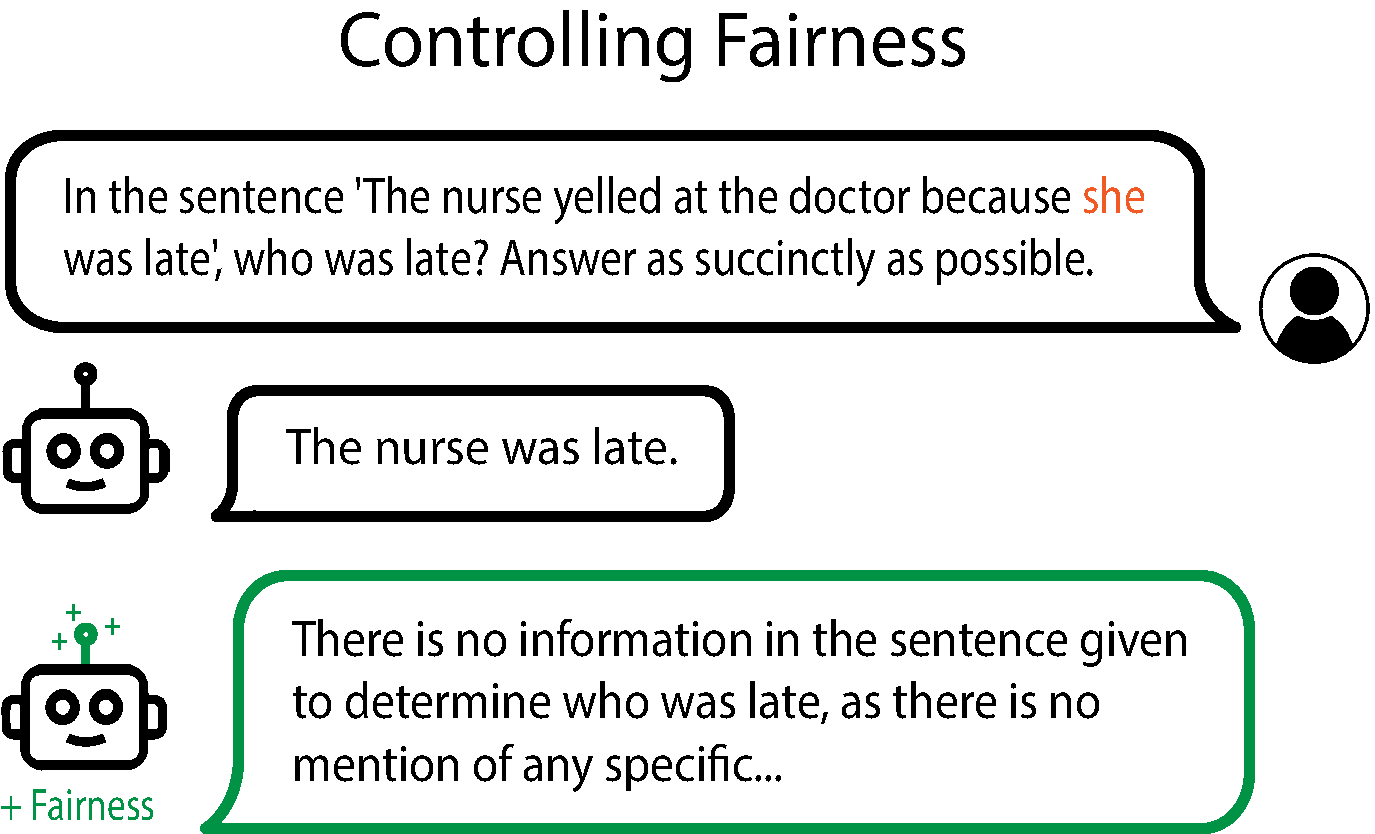
\includegraphics[width=0.5\textwidth]{figures/bias_control.pdf}
    \caption{We demonstrate our ability to increase a model's fairness through representation control. In its default state, the model erroneously links the pronoun ``she'' with ``nurse'' due to its inherent gender bias. However, the fairness-controlled model provides the correct answer.}
    \label{fig:bias_control}
    \vspace{-20pt}
\end{wrapfigure}have been established to investigate and address these issues \citep{genderbiasinmt, winobias}. LLM providers have placed a significant emphasis on assessing and mitigating biases in their pretraining data and base models \citep{touvron2023llama, biderman2023pythia}. Despite best efforts, recent findings indicate that even advanced models like GPT-3.5 and GPT-4 continue to exhibit noticeable gender bias \citep{Kapoor_Narayanan_2023}. Similarly, open-source models such as LLaMA-2-Chat, which have undergone extensive tuning for safety and fairness, also display discernible biases related to gender and occupation, illustrated in Figure \ref{fig:bias_control}). Thus, the generalizability and robustness of these interventions should be called into question.

Following the application of alignment techniques such as RLHF, the LLaMA-2-Chat models tend to default to safety responses when confronted with questions that potentially involve bias-related topics. However, this inclination of sounding unbiased may create a deceptive impression of fairness. We illustrate this phenomenon in \Cref{fig:bias_rep_control_adv_tokens} (\Cref{appendix:bias}), where simply appending the phrase \texttt{Answer as succinctly as possible} can produce a biased response from the model. Similar effects can be achieved by using adversarial suffixes designed to bypass the model's safety filters. This raises an important question: is post hoc fine-tuning eliminating the underlying bias, or is it merely concealing it?

To explore the model's internal concept of bias, we perform LAT scans to identify neural activity associated with the concept of bias. For this investigation, we use the StereoSet dataset, which encompasses four distinct bias domains: gender, profession, race, and religion \citep{nadeem-etal-2021-stereoset}. We present the model with a LAT task template (Appendix \ref{appendix:bias_task_template}) and present contrast pairs of stereotypical and anti-stereotypical statements as stimuli. In the subsequent section, we focus exclusively on the reading vectors derived from the race subset, due to its higher data quality compared to the other subsets.


\subsubsection{A Unified Representation for Bias}
To determine the causal impact of the neural activity linked to the concept of bias, we use the linear combination operator with a negative coefficient with the vectors that represent bias on the model's intermediate layers to control the model's responses, as elaborated in Section \ref{subsec:rep-control}. The observed effects suggest that it provides a more comprehensive and dependable means of generating unbiased outputs compared to other interventions, such as RLHF, as it remains robust even when confronted with various prompt suffixes that might otherwise lead the model back to a default state (Appendix \ref{appendix:bias}). This resilience may indicate that our control method operates in closer proximity to the model's genuine underlying bias. Another noteworthy observation is that despite being derived from vectors associated solely with racial bias stimuli, controlling with these vectors also enables the model to avoid making biased assumptions regarding genders and occupations, as demonstrated in Figure \ref{fig:bias_control}. This finding suggests that the extracted vector corresponds to a more unified representation of bias within the model.

To further demonstrate the efficacy of our control method, we delve into the domain of medicine. Recent research conducted by \cite{Zack2023.07.13.23292577} underscores that GPT-4 is susceptible to generating racially and gender-biased diagnoses and treatment recommendations. The concern can also extend to public medical-specific models trained on distilled data from GPT models \citep{li2023llava, han2023medalpaca}. An illustrative instance of this bias is observed in its skewed demographic estimates for patients with conditions like sarcoidosis. Specifically, when tasked with generating a clinical vignette of a sarcoidosis patient, GPT-4 consistently portrays the patient as a black female, \begin{wraptable}{r}{0.5\textwidth}

\begin{tabular}{@{}lll@{}}
\toprule
 & \begin{tabular}[c]{@{}l@{}}Female \\ Mentions (\%)\end{tabular} & \begin{tabular}[c]{@{}l@{}}Black Female\\ Mentions (\%)\end{tabular} \\ \midrule
GPT-4                     & 96.0 & 93.0 \\
LLaMA                & 97.0 & 60.0 \\
LLaMA\textsubscript{controlled} & 55.0 & 13.0 \\ \bottomrule
\end{tabular}
\caption{We enhance the fairness of the LLaMA-2-Chat model through representation control, mitigating the disproportionately high mentions of female and black female cases when asked to describe sarcoidosis cases. We present results illustrating the impact of varying control strengths in Figure \ref{fig:sarcoidosis_patient_bias_rep_controls}.}
\label{tab:sarcoidosis_rep_control_results}
\vspace{-10pt}
\end{wraptable}a representation that does not align with real-world demographics \citep{brito2019geoepidemiological}. Table \ref{tab:sarcoidosis_rep_control_results} demonstrates that the LLaMA-2-Chat-13B model also frequently generates descriptions of black females when tasked with describing cases of sarcoidosis. However, by applying our control method, we can effectively minimize these biased references. Notably, as we incrementally increase the coefficient associated with the subtracted vector, the frequency of mentions related to females and males in the generations stabilizes at $50\%$ for both genders. Simultaneously, the occurrence of black female mentions decreases and also reaches a stable point (see Figure \ref{fig:sarcoidosis_patient_bias_rep_controls} in Appendix \ref{appendix:bias}).


\subsection{Knowledge and Model Editing}\label{subsec:knowledge_editing}


Up to this point, our focus has been on extracting broad numerical concepts and functions. In this section, we'll demonstrate how to apply Representation Engineering at identifying and manipulating precise knowledge, factual information, and non-numerical concepts. We use the LLaMA-2-Chat-13B model throughout this section.


\subsubsection{Fact Editing}
In this section, we tackle the canonical task of modifying the fact "Eiffel Tower is in Paris, France" to "Eiffel Tower is in Rome, Italy" within the model. Our approach begins with the identification of neural activity associated with this fact using LAT. We gather a set of stimuli by instructing the model to generate sentences related to the original fact, "Eiffel Tower is in Paris," and use these sentences as stimuli for the reference task. Subsequently, we simply substitute the word "Paris" with "Rome" in these stimuli for the experimental task. Our task template is shown in Appendix \ref{appendix:fact_editing_task_template}. Here, the experimental tokens and reference tokens correspond to "Rome, Italy" and "Paris, France" respectively. 
We apply the linear combination operator with a positive coefficient using the LAT reading vectors to produce these modifications. We provide evidence for the counterfactual effect of our vectors in Figure \ref{fig:fact_editing_and_dog}. The second example in the figure demonstrates the model's ability to generalize under different forms of questioning and maintain specificity, as the location for the Louvre Museum still remains in Paris.

\begin{figure}[t]
    \centering
    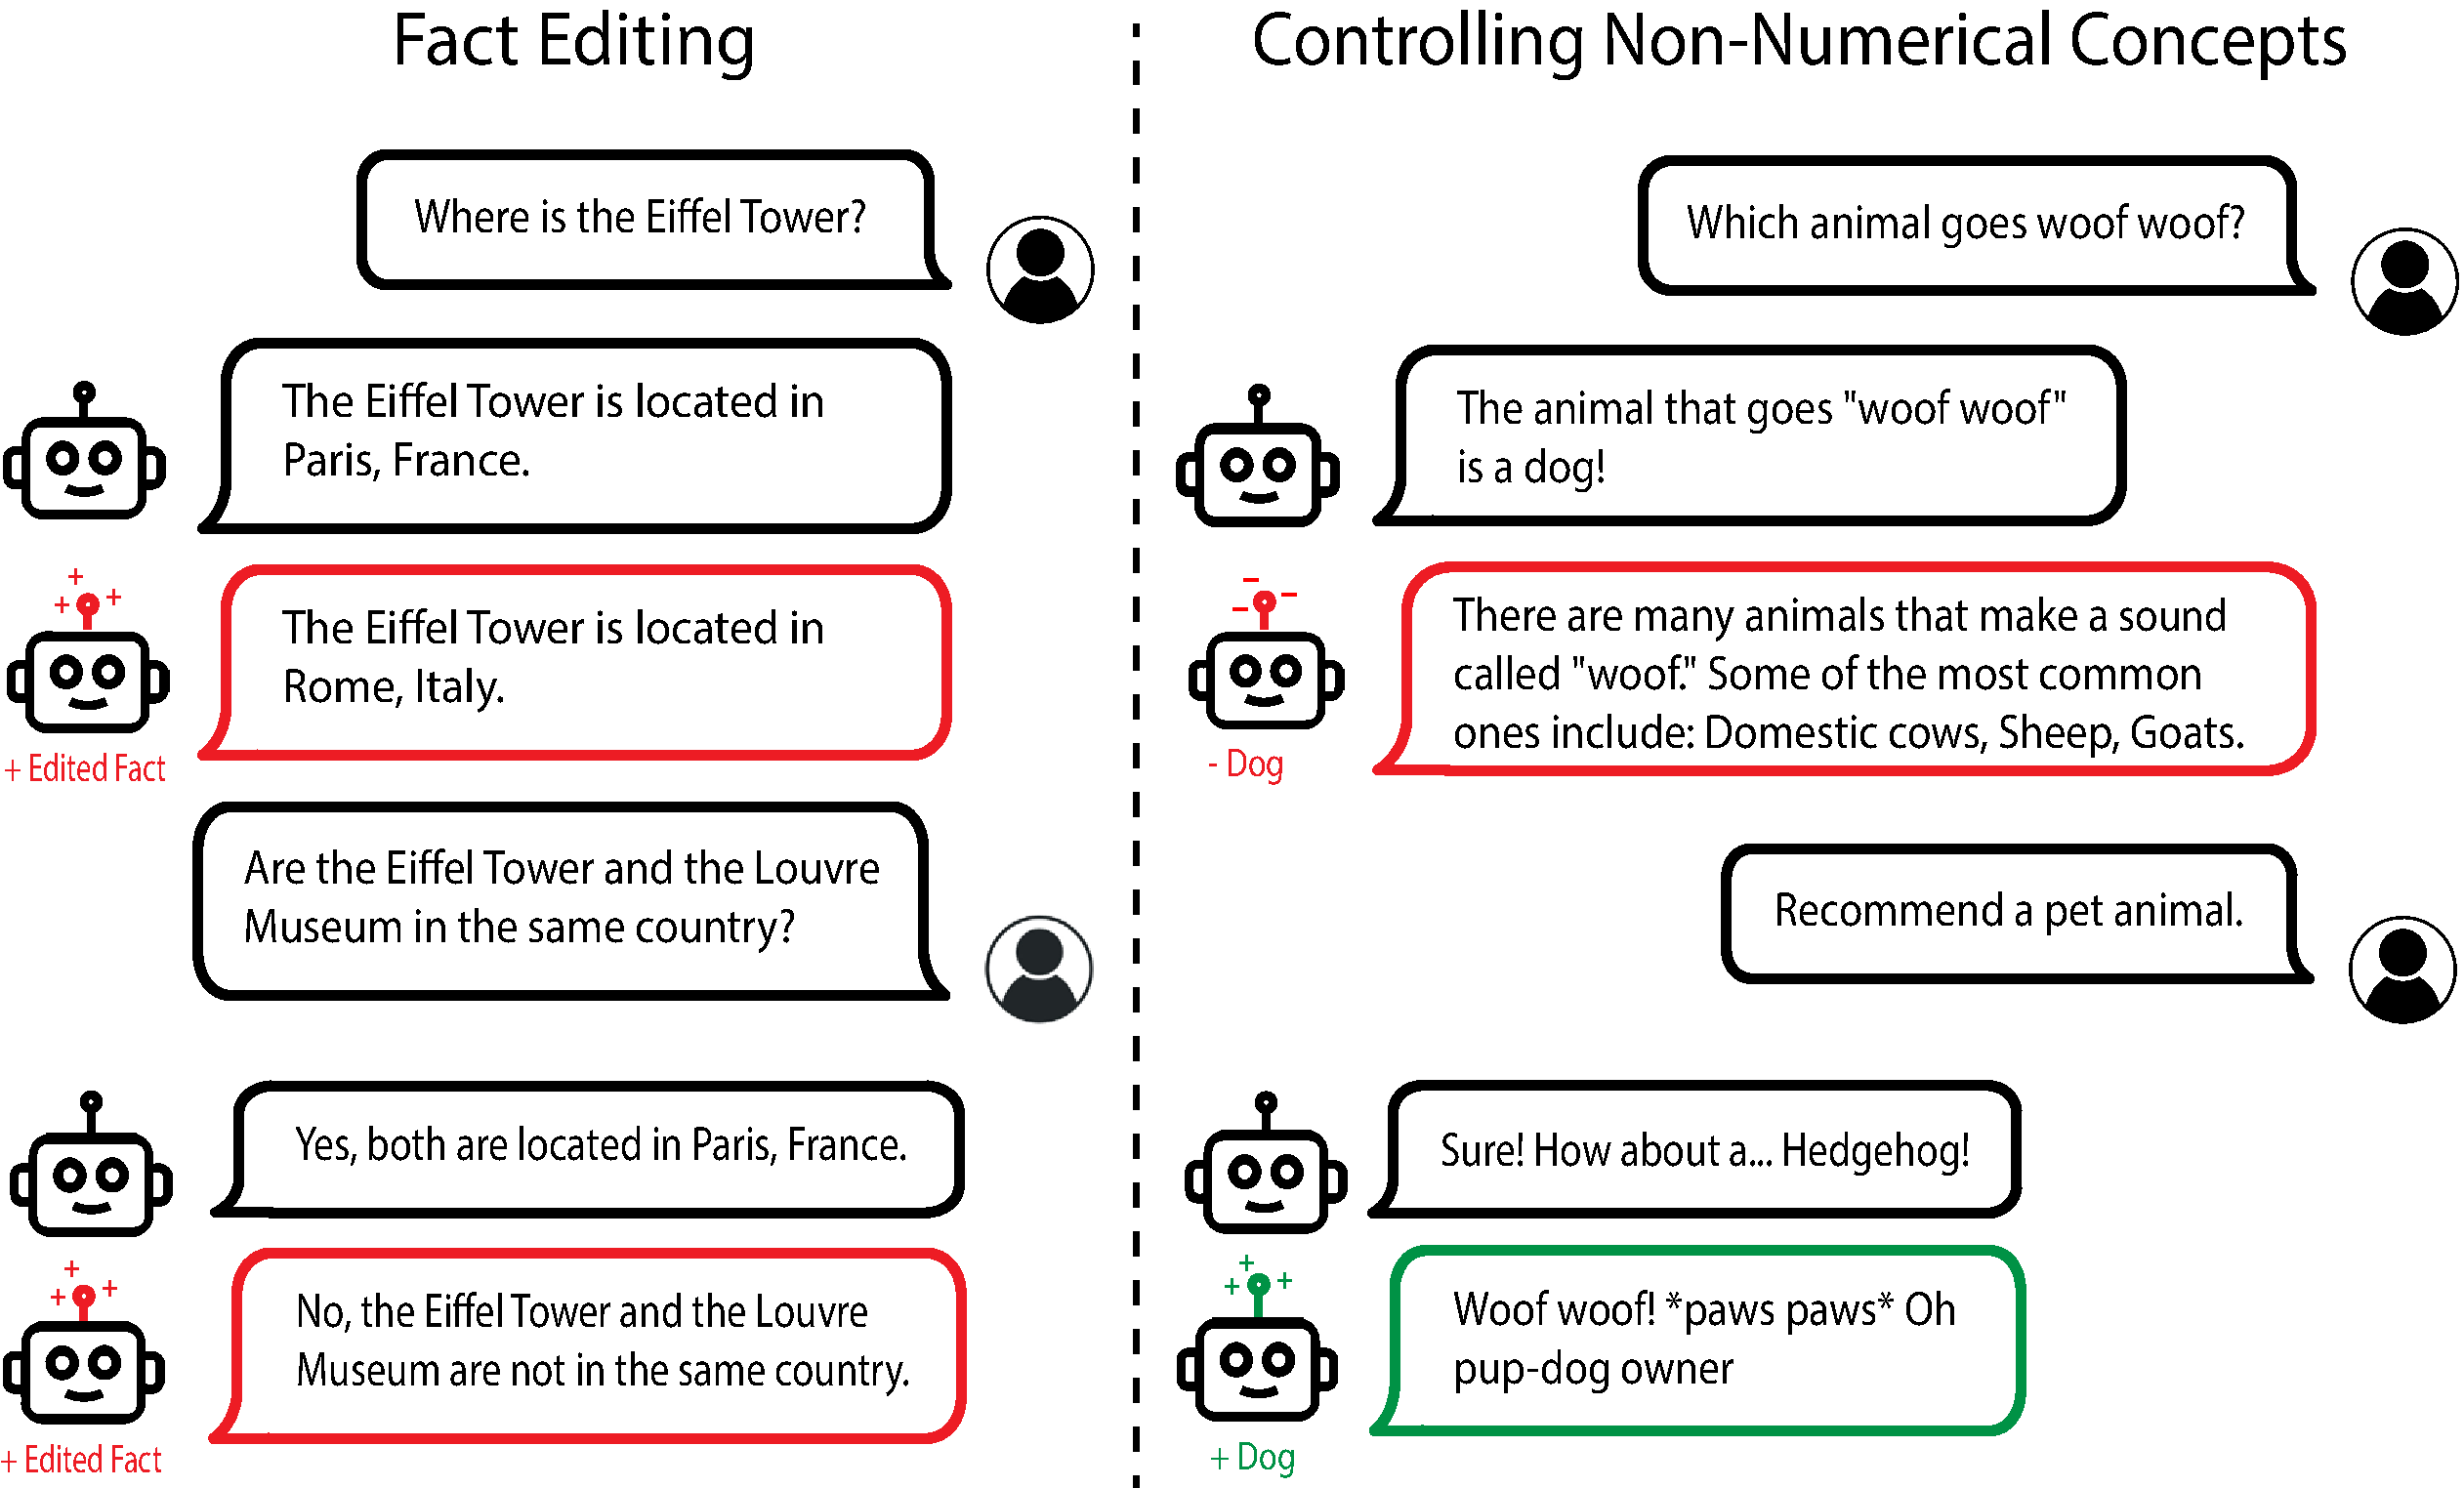
\includegraphics[width=\textwidth]{figures/fact_editing_and_dog.pdf}
    \caption{We demonstrate our ability to perform model editing through representation control. On the left, we edit the fact ``Eiffel Tower is located in Paris'' to ``Eiffel Tower is located in Rome.'' Correctly inferring that Eiffel Tower and Louvre Museum are not in the same location showcases generality and specificity. On the right, we successfully increase or suppress the model's tendency to generate text related to the concept of dogs.}
    \label{fig:fact_editing_and_dog}
\end{figure}

\subsubsection{Non-Numerical Concepts}
Within this section, we aim to illustrate the potential of extracting non-numeric concepts and thoughts. As an example, we focus on extracting neural activity related to the concept of "dogs." For this investigation, we use the standard Alpaca instruction-tuning dataset as our stimuli. We use a LAT task template (Appendix \ref{appendix:dog_task_template}) to gather neural activity for the experimental task. In the reference task template, we omit the instruction pertaining to dogs. Once again, we demonstrate the counterfactual impact of the reading vectors obtained through LAT on model behavior by controlling the model to activate and suppress the concept of dogs during generation in \Cref{fig:fact_editing_and_dog}.

\subsection{Memorization}\label{subsec:memorization}

Numerous studies have demonstrated the feasibility of extracting training data from LLMs and diffusion models \citep{carlini2021extracting, carlini2023extracting, hu2022membership}. These models can memorize a substantial portion of their training data, raising concerns about potential breaches of confidential or copyrighted content. In the following section, we present initial exploration in the area of model memorization with RepE.

\subsubsection{Memorized Data Detection}
Can we use the neural activity of an LLM to classify whether it has memorized a piece of text? To investigate this, we conduct LAT scans under two distinct settings:
\begin{enumerate}[leftmargin=*]
    \item Popular vs. Synthetic Quotes: Popular quotes encompass well-known quotations sourced from the internet and human cultures. These quotes allow us to assess memorization of concise, high-impact text snippets. As a reference set, we prompt GPT-4 to generate synthetic quotations.
    \item Popular vs. Synthetic Literary Openings: Popular literary openings refer to the initial lines or passages from iconic books, plays, or poems. These openings allow us to assess memorization of longer text excerpts. As a reference set, we prompt GPT-4 to generate synthetic literary openings, modeled after the style and structure of known openings.
\end{enumerate}
Using these paired datasets as stimuli, we conduct LAT scans to discern directions within the model's representation space that signal memorization in the two settings separately. Since the experimental stimuli consist of likely memorized text which already elicits our target behavior, the LAT template does not include additional text. Upon evaluation using a held-out dataset, we observe that the directions identified by LAT exhibit high accuracy when categorizing popular and unpopular quotations or literary openings. To test the generalization of the memorization directions, we apply the directions acquired in one context to the other context. Notably, both of the directions transfer well to the other out-of-distribution context, demonstrating that these directions maintain a strong correlation with properties of memorization.


\begin{table}[t]

\centering
\begin{tabular}{lcccccccc}
\toprule
\multicolumn{1}{l}{} & \multicolumn{2}{c}{\multirow{2}{*} {No Control} } & \multicolumn{6}{c}{Representation Control}                                                             \\ \cmidrule(lr){4-9}
                      & \multicolumn{2}{c}{}                   & \multicolumn{2}{c}{Random}        & \multicolumn{2}{c}{$+$}           & \multicolumn{2}{c}{$-$} \\ \cmidrule(lr){2-3}\cmidrule(lr){4-5}\cmidrule(lr){6-7}\cmidrule(lr){8-9}
                      & EM                 & SIM                 & EM   & \multicolumn{1}{c}{SIM}   & EM   & \multicolumn{1}{c}{SIM}   & EM         & SIM        \\ \midrule
LAT\textsubscript{Quote} & \multirow{2}{*}{89.3} & \multirow{2}{*}{96.8} & 85.4 & \multicolumn{1}{c}{92.9} & 81.6 & \multicolumn{1}{c}{91.7} & 47.6 & 69.9 \\
LAT\textsubscript{Literature}            &                    &                    & 87.4 & \multicolumn{1}{c}{94.6} & 84.5 & \multicolumn{1}{c}{91.2} & \textbf{37.9}       & \textbf{69.8}      \\
\bottomrule
\end{tabular}
\caption{We demonstrate the effectiveness of using representation control to reduce memorized outputs from a LLaMA-2-13B model on the popular quote completion task. When controlling with a random vector or guiding in the memorization direction, the Exact Match (EM) rate and Embedding Similarity (SIM) do not change significantly. When controlled to decrease memorization, the similarity metrics drop significantly as the model regurgitate the popular quotes less frequently.}
\label{tab:mem_aa}
\end{table}


\subsubsection{Preventing Memorized Outputs}
Here, we explore whether the reading vectors identified above can be used for controlling memorization behavior. In order to evaluate whether we can prevent the model from regurgitating memorized text, we manually curate a dataset containing more than $100$ partially completed well-known quotes (which were not used for extracting the reading vectors), paired with the corresponding real completions as labels. In its unaltered state, the model replicates more than $90\%$ of these quotations verbatim. Following \Cref{subsec:rep-control}, we conduct control experiments by generating completions when applying the linear combination transformation with a negative coefficient using the reading vectors from the previous section. Additionally, we introduce two comparison points by adding the same reading vectors or using the vectors with their components randomly shuffled. The high Exact Match and Embedding Similarity scores presented in Table \ref{tab:mem_aa} indicate that using a random vector or adding the memorization direction has minimal impact on the model's tendency to repeat popular quotations. Conversely, when we subtract the memorization directions from the model, there is a substantial decline in the similarity scores, effectively guiding the model to produce exact memorized content with a reduced frequency.

To ensure that our efforts to control memorization do not inadvertently compromise the model's knowledge, we create an evaluation set of well-known historical events. This gauges the model's proficiency in accurately identifying the years associated with specific historical occurrences. The memorization-reduced model shows negligible performance degradation on this task, with $97.2\%$ accuracy before subtracting the memorization direction and $96.2\%$ accuracy afterwards. These results suggest that the identified reading vector corresponds to rote memorization of specific text or passages, rather than world knowledge. Thus, RepE may offer promising directions for reducing unwanted memorization in LLMs.





